\begin{figure}
	\centering
	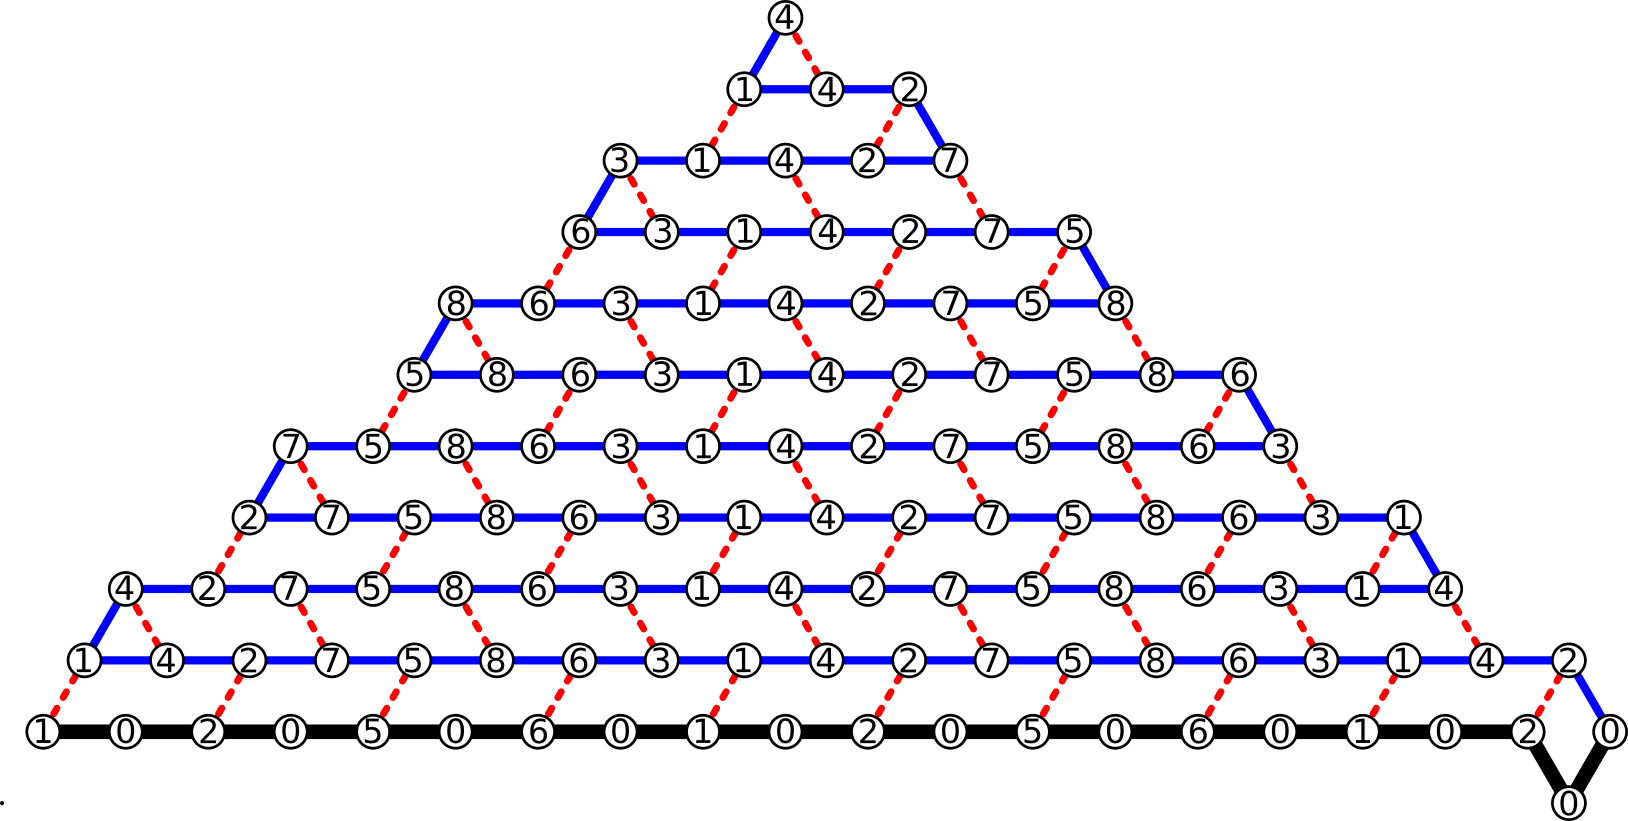
\includegraphics[width=0.7\linewidth]{./Fig/CI_NumbersNew}
	\caption{Quadratic length transcript folding deterministically into pyramid shape. Seed: thick black path. Transcript: thin blue path. Bonds: dashed red lines. }
	\label{CI:big}
\end{figure}

%\subsection{$\alpha = 1$, arbitrary alphabets}
First we present a lower bound construction for arity $1$ systems. At $\alpha=1$, having delay $\delta=2$ allows the deterministic folding of quadratic length transcripts compared with $\delta=1$, where, as stated before, the maximum length is linear in the length of the seed. We demonstrate this with an infinite family of OS, which fold deterministically a transcript of length $\frac{(n-1)^2}{4}$ starting from a given seed of length $n$.



Consider the following $\delta=2$, $\alpha=1$ system with bead types $\{0,1,\dots,8\}$ and attraction rules $\{(i,i) \mid 1\leq i\leq 8\}$. Let the seed $\sigma$ be a conformation of a $4k+1$ long bead sequence of the form $(10205060)^{k/2}0$ and $(10205060)^{(k-1)/2}(1020)0$, for $k$ even and odd, respectively. Bead $\sigma[i]$ of the seed is stabilized at point $(i,0)$, for all $1\leq i\leq 4k-1$. Bead $4k$ is at $(4k-1,-1)$ and bead $4k+1$ is at $(4k,0)$.
\vspace{0.1cm}

The transcript is $w=\mathrm{row}_1\cdots \mathrm{row}_{2k}$, where 
\begin{itemize}
	\item $\mathrm{row}_1=(24136857)^{(k-1)/2}241$ if $k$ is odd, and $\mathrm{row}_1=(68572413)^{k/2-1}6857241$ if $k$ is even;
	\item $\mathrm{row}_{i+1}=(\mathrm{row}_i[2..|\mathrm{row}_i|-1])^r$ for $i\in \{1,\dots, 2k-1\}$, where $w^r$ is the reverse of $w$. In other words, each row is the reverse of the previous without its first and last bead.
\end{itemize}


%The transcript is $w=\mathrm{row}_1\cdots \mathrm{row}_{2k}$, where $\mathrm{row}_\ell$, for $\ell\in \{1,\dots, 2k\}$ is given in the table of Fig.~\ref{table:transcript}.
%\begin{figure}[h]
%%	\begin{minipage}{.49\textwidth}
%%		%\centering
%%		\begin{tabular}{l|l}
%%			\multicolumn{2}{c}{Transcript $w$}\\
%%			\multicolumn{2}{c}{}  \\
%%			$k$ odd & \hspace{0.3cm} $k$ even\\\hline
%%			& \\
%%			$(24136857)^{(k-1)/2}241$\hspace{0.3cm} & \hspace{0.3cm} $(2413)^{k-1}241$\\
%%			$42(75863142)^{k-1}314$   &  \hspace{0.3cm} $(4231)^{k-1}4$  \\
%%			$13(68572413)^{k-2}2$ &  \hspace{0.3cm} $(1324)^{k-2}132$\\
%%			$(3142)^{k-2}3$   &  \hspace{0.3cm} $(3142)^{k-2}3$ \\
%%			\vdots			 &  \hspace{0.3cm} \vdots\\
%%			$(1324)^1 132$	 &  \hspace{0.3cm} $(2413)^{1} 241$\\
%%			$(3142)^1 3$		 & \hspace{0.3cm} $(4231)^1 4$\\
%%			$(2413)^0 241$	 &  \hspace{0.3cm} $(1324)^0 132$\\
%%			$(4231)^0 4$		 & \hspace{0.3cm} $(3142)^0 3$\\
%%		\end{tabular}
%%	\end{minipage}
%	%\scriptsize
%	\begin{minipage}{.99\textwidth}
%		\centering
%		\begin{tabular}{|l|c|}
%			\hline
%			\hspace{1.2cm}row $\ell$ & $\ell\mod 4$ \\\hline
%			 & \\
%			\hspace{0.1cm}$(24136857)^{k-\lfloor (\ell+1)/2\rfloor}241$ \hspace{0.1cm} &  $\textrm{ }\ell\equiv 1\mod 4\textrm{ }$\\
%			\hspace{0.1cm}$(4231)^{k-\lfloor (\ell+1)/2\rfloor}4$   &  $\textrm{ }\ell\equiv 2 \mod 4\textrm{ }$ \\
%			\hspace{0.1cm}$(1324)^{k-\lfloor (\ell+1)/2\rfloor}132$ &  $\textrm{ }\ell\equiv 3 \mod 4\textrm{ }$ \\
%			\hspace{0.1cm}$(3142)^{k-\lfloor (\ell+1)/2\rfloor}3$   &  $\textrm{ }\ell\equiv 4 \mod 4\textrm{ }$ \\\hline
%		\end{tabular}
%	
%	\end{minipage}
%	\caption{Transcript of pyramid-like conformation at delay $2$, arity $1$.}
%	\label{table:transcript}
%\end{figure}

The transcript above is written in rows which correspond to beads in the conformation stabilized along the same row on the grid. To simplify the argument we will use \textit{row} both for the transcript above and for the conformation it stabilizes in (note that in the figure the row index grows from bottom to top). 

Row $1$ is of length $4k-1$ and row $\ell+1$ is two beads shorter than row $\ell$, so the length of the whole transcript is $|w|=4k^2=\frac{(4k+1-1)^2}{4}=\frac{(|\sigma|-1)^2}{4}$. As an example, see Fig.~\ref{CI:big}, where $k=5$, so the length of the seed is $4k+1=21$ and the transcript is $4k^2 = 100$ beads long.




Stabilizing the first bead of a row goes by binding to the penultimate bead of the previous row, as they are of the same type according to how we constructed the transcript, and they have free hands (see Fig.~\ref{CI:turn}).
%\begin{itemize}
%	\item $\bf j\equiv 1\mod 4$: the first two beads are $24$, and the preceding bead is stabilized at $(4k-\frac{j-1}{2}, j-1)$. The $2$ can only bind to the $2$ which occurred two beads before at $(4k-\frac{j+1}{2}, j-1)$, and $4$ cannot bind anywhere, so the $2$ is stabilized at $(4k-\frac{j-1}{2},j)$.
%\end{itemize}

%\begin{center}
%	\begin{tabular}{|c|c|c|c|c|@{}m{0pt}@{}}
%		%\renewcommand{\arraystretch}{2}
%	$j\mod 4$					& first bead 	& predecessor at		& first bead binds to		& first stabilizes at\\
%						\hline
%	$\equiv 1$	& 2		& $(4k-\frac{j-1}{2}, j-1)$		& $(4k-\frac{j+1}{2}, j-1)$	& $(4k-\frac{j+1}{2}, j)$& $\mathrm{ }$\newline $\mathrm{ }$\\
%	\hline
%	$\equiv 2$	& 4				& $(\frac{3j}{2}-1,j-1)$		& $(\frac{3j}{2},j-1)$		& $(\frac{3j}{2},j)$ & $\mathrm{ }$\newline $\mathrm{ }$\\
%	\hline
%	$\equiv 3$	& 1				& $(4k-\frac{j-1}{2}, j-1)$		& $(4k-\frac{j+1}{2}, j-1)$	& $(4k-\frac{j+1}{2}, j)$ & $\mathrm{ }$\newline $\mathrm{ }$ \\
%	\hline
%	$\equiv 4$	& 3				& $(\frac{3j}{2}-1,j-1)$		& $(\frac{3j}{2},j-1)$		& $(\frac{3j}{2},j)$ & $\mathrm{ }$\newline $\mathrm{ }$ \\
%	\hline		
%	\end{tabular}
%\end{center}



%The first bead of the transcript is type $2$ and it has to be fixed next to $(4k,0)$. The second bead is type $4$, which cannot form a bond with anything in the conformation so far. The only possibility of forming a bond is if the $2$-bead is placed at $(4k,1)$ and it bonds with the $2$-bead of the seed at $(4k-1,0)$. The next to be stabilized is a $4$-bead, and since it cannot form any bond, the conformation with the highest number of bonds is when the one after, a $1$-bead, is at $(4k-2,1)$ bonding with $(4k-3,0)$, which stabilizes the preceding $4$-bead at $(4k-1,1)$ (see Fig.~\ref{CI:1-4}, (a)-(b)).



\begin{figure}
	\begin{minipage}{.35\textwidth}
		\centering
		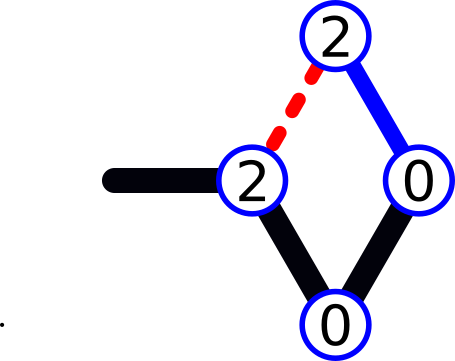
\includegraphics[align=c,height=1in]{./Fig/CI_1n}\\
		\bigskip
		
		(a) First transcript bead 
	\end{minipage}%
	\begin{minipage}{.2\textwidth}
		\centering
		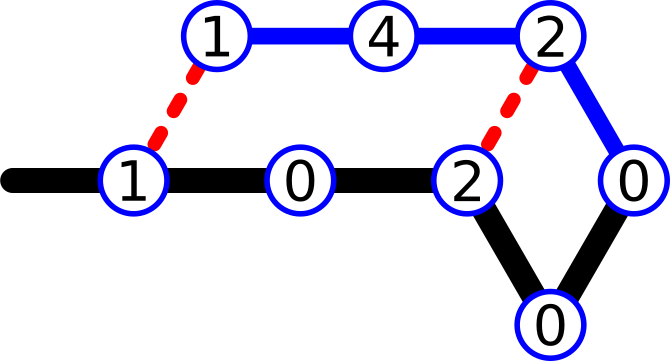
\includegraphics[align=c,height=0.7in]{./Fig/CI_2n}\\
		\bigskip
		
		(b) Second bead
	\end{minipage}
	\begin{minipage}{.4\textwidth}
		\centering
		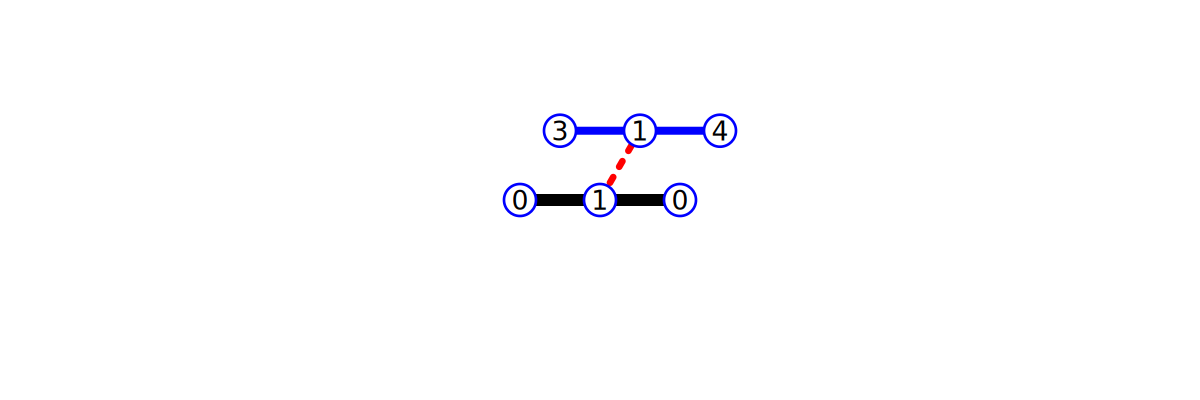
\includegraphics[align=c,height=0.5in]{./Fig/CI_3n}
		\bigskip
		\vspace{0.1in}
		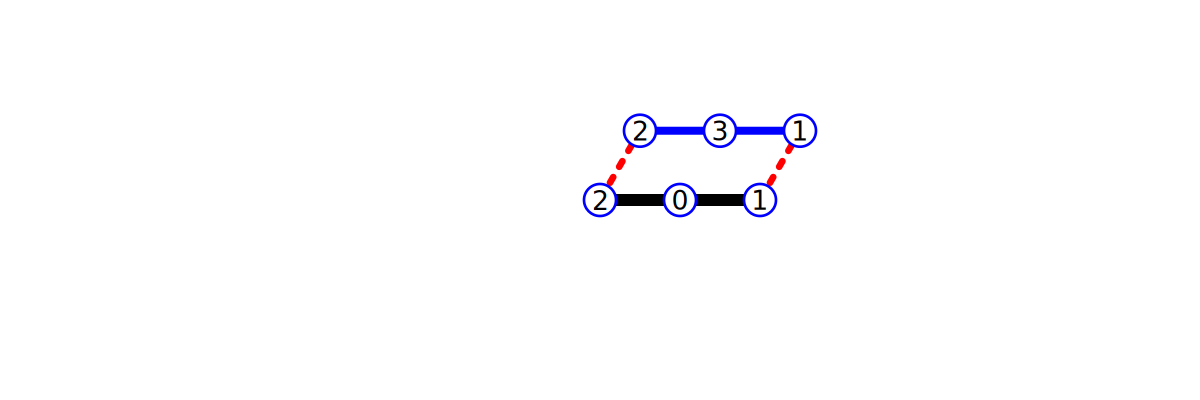
\includegraphics[align=c,height=0.5in]{./Fig/CI_4n}
		\bigskip
		
		(c) Portions of row $1$
	\end{minipage}
	\caption{Fixing transcript beads in first row, when $k$ is odd}
	\label{CI:1-4}
\end{figure}


As for the other beads, in rows $j\equiv 1,3\mod 4$, beads of type $1,2,5,6$ bind to a bead in row $j-1$. In rows $j\equiv 2,4\mod 4$ beads of type $3,4,7,8$ can bind to a bead in row $j-1$.  This is true for row $1$, because beads of type $1,2,5,6$ from row $1$ can only bind to every second bead of the seed, whereas the other beads of row $1$ cannot bind to anything (Fig.~\ref{CI:1-4}, (c)). Once this dynamic holds for a row, it holds inductively for the next, as a bead that binds to another loses its only free hand at arity $1$.

Within one row of the transcript, no bead $i$ can bind to a preceding bead, because if there is a previous bead of the same type in that row, it is stabilized at a distance of at least $6$ from any point where $i$ could be placed.

By the arguments above, the beads in row $i$ of the transcript are stabilized along row $i$ on the grid, forming the pyramid-like conformation from Fig.~\ref{CI:big}.


\begin{figure}
	\centering
	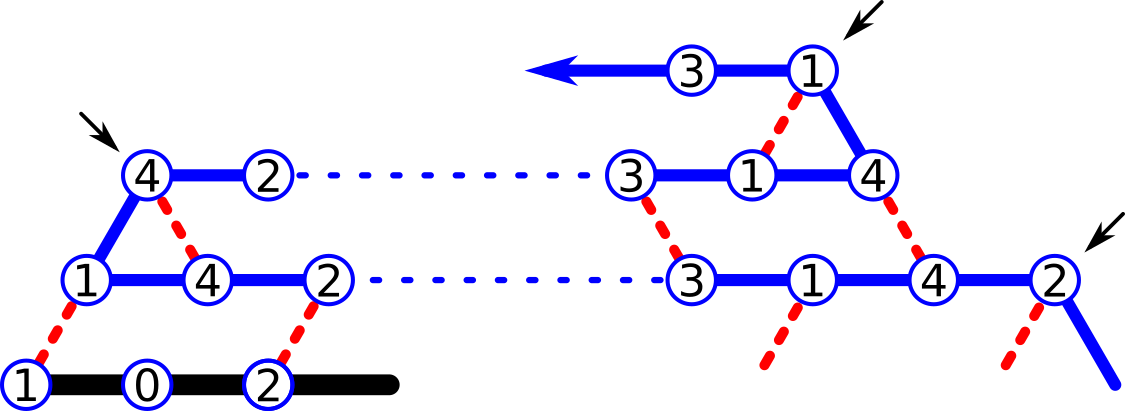
\includegraphics[width=0.7\linewidth]{./Fig/CI_turnn}
	\caption{Beads $4k, 8k-2, \dots$ stabilize at turning points because the bead two positions before is the same type and has a free hand.}
	\label{CI:turn}
\end{figure}



